\documentclass[legalpaper]{article}
\usepackage{lscape}
\usepackage{tikz}
\usetikzlibrary{arrows,shapes,positioning,shadows,trees}

\tikzset{
  basic/.style  = {draw, text width=20em, drop shadow, font=\sffamily, rectangle},
  root/.style   = {basic, rounded corners=2pt, thin, align=center,
                   fill=green!30},
  level 2/.style = {basic, rounded corners=6pt, thin,align=center, fill=green!60,
                   text width=10em},
  level 3/.style = {basic, thin, align=left, fill=pink!60, text width=15em}
}

\begin{document}
\begin{landscape}
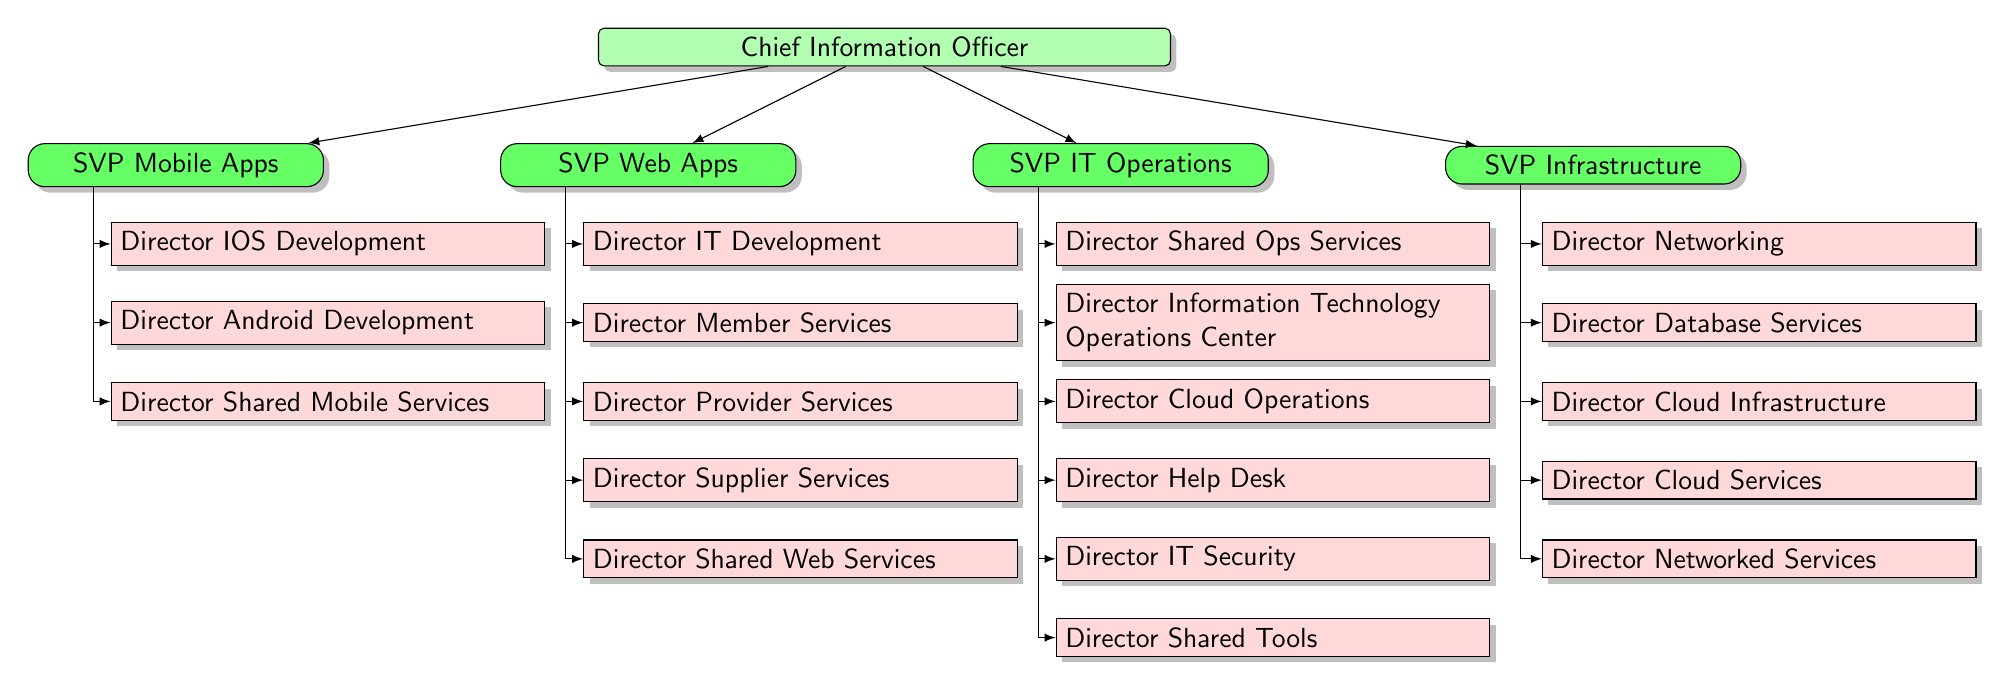
\begin{tikzpicture}[
  level 1/.style={sibling distance=60mm},
  edge from parent/.style={->,draw},
  >=latex]

% root of the the initial tree, level 1
\node[root] {Chief Information Officer}
% The first level, as children of the initial tree
  child {node[level 2] (c1) {SVP Mobile Apps}}
  child {node[level 2] (c2) {SVP Web Apps}}
  child {node[level 2] (c3) {SVP IT Operations}}
  child {node[level 2] (c4) {SVP Infrastructure}};

% The second level, relatively positioned nodes
\begin{scope}[every node/.style={level 3}]
\node [below of = c1, xshift=55pt] (c11) {Director IOS Development};
\node [below of = c11] (c12) {Director Android Development};
\node [below of = c12] (c13) {Director Shared Mobile Services};

\node [below of = c2, xshift=55pt] (c21) {Director IT Development};
\node [below of = c21] (c22) {Director Member Services};
\node [below of = c22] (c23) {Director Provider Services};
\node [below of = c23] (c24) {Director Supplier Services};
\node [below of = c24] (c25) {Director Shared Web Services};

\node [below of = c3, xshift=55pt] (c31) {Director Shared Ops Services};
\node [below of = c31] (c32) {Director Information Technology Operations Center};
\node [below of = c32] (c33) {Director Cloud Operations};
\node [below of = c33] (c34) {Director Help Desk};
\node [below of = c34] (c35) {Director IT Security};
\node [below of = c35] (c36) {Director Shared Tools};

\node [below of = c4, xshift=60pt] (c41) {Director Networking};
\node [below of = c41] (c42) {Director Database Services};
\node [below of = c42] (c43) {Director Cloud Infrastructure};
\node [below of = c43] (c44) {Director Cloud Services};
\node [below of = c44] (c45) {Director Networked Services};

\end{scope}

% lines from each level 1 node to every one of its "children"
\foreach \value in {1,2,3}
  \draw[->] (c1.195) |- (c1\value.west);

 \foreach \value in {1,...,5}
   \draw[->] (c2.195) |- (c2\value.west);

 \foreach \value in {1,...,6}
   \draw[->] (c3.195) |- (c3\value.west);

 \foreach \value in {1,...,5}
   \draw[->] (c4.195) |- (c4\value.west);

\end{tikzpicture}
\end{landscape}
\end{document}
